\documentclass[12pt,a4paper]{article}
\usepackage[utf8]{inputenc}
\usepackage{graphicx}
\usepackage{hyperref}
\usepackage{geometry}
\usepackage{float}
\usepackage{titlesec}
\usepackage{tikz}
\usetikzlibrary{shapes.geometric, arrows, positioning, fit, calc}

\geometry{a4paper, margin=1in, headheight=15pt}
\usepackage{fancyhdr}
\usepackage{tabularx}
\usepackage{array}

\pagestyle{fancy}
\fancyhf{}
\fancyhead[L]{FraudGuard DevOps Platform}
\fancyhead[R]{CSE 816 Evaluation Report}
\renewcommand{\headrulewidth}{0.4pt}

\begin{document}

\begin{titlepage}
    \thispagestyle{empty}
    \centering
    \vspace*{1cm}
    
    {\huge \textbf{FraudGuard DevOps Platform} \par}
    \vspace{0.5cm}
    {\large FinTech + AIOps/MLOps Integrated DevOps Pipeline \par}
    
    \vspace{1.5cm}
    \rule{\linewidth}{0.8pt}\\[0.5cm]
    {\Huge \textbf{Project Evaluation Report}}\\[0.5cm]
    \rule{\linewidth}{0.8pt}
    \vspace{2cm}
    
    \begin{table}[H]
        \centering
        \renewcommand{\arraystretch}{1.2}
        \begin{tabular}{lp{10cm}}
            \textbf{Course} & CSE 816 - Software Production Engineering \\
            \textbf{Team Members} & Kautilya Singh (MT2025064) \\
            & Vishesh Tamrakar (MS2025021) \\
            \textbf{Project} & FraudGuard DevOps Platform \\
            \textbf{Submission Type} & End-to-End DevOps + MLOps Evaluation \\
            \textbf{Platform} & Ubuntu 24.04 LTS (Native Minikube, no VM) \\
            \textbf{Date} & May 14, 2026 \\
            \textbf{Repository} & \url{https://github.com/Vishesh-tamrakar/Fraudguard-devops}
        \end{tabular}
    \end{table}
    
    \vfill
    
    \begin{center}
    {\normalsize This report summarizes architecture, implementation, deployment, observability, and \\ validation evidence for the FraudGuard DevOps Platform. \par}
    \end{center}
    \vspace{1cm}
\end{titlepage}

\newpage
\thispagestyle{fancy}
\tableofcontents
\newpage

\section{System Overview}
FraudGuard is an advanced, production-grade MLOps platform designed to provide real-time fraud detection for financial transactions. By integrating a custom-trained machine learning model within a highly scalable DevOps pipeline, the platform bridges the gap between data science and operational software engineering. The system ensures high availability, automated deployments, secure secrets management, and comprehensive observability. It aligns perfectly with the requirements of the CSE 816 Final Project by fulfilling all core DevOps criteria and advanced MLOps domain requirements.

\begin{figure}[H]
    \centering
    \includegraphics[width=0.9\textwidth]{Screenshots/Specifications.png}
    \caption{System Environment and Specifications}
\end{figure}

\subsection{End-to-End Execution Sequence}
The DevOps lifecycle is designed for end-to-end automation. The sequence of execution from a code change to production observability is illustrated below. 

\newpage

When a developer pushes code to GitHub, a webhook immediately triggers Jenkins. Jenkins orchestrates the pipeline: it runs Ansible to ensure the Kubernetes environment is provisioned, builds the Docker image containing the ML model, fetches Docker Hub credentials securely from Vault, pushes the image, and deploys it to Kubernetes. Once running in Kubernetes, the application is monitored by the HPA and logs are automatically shipped to the ELK stack.

\begin{figure}[H]
\centering
\resizebox{\textwidth}{!}{%
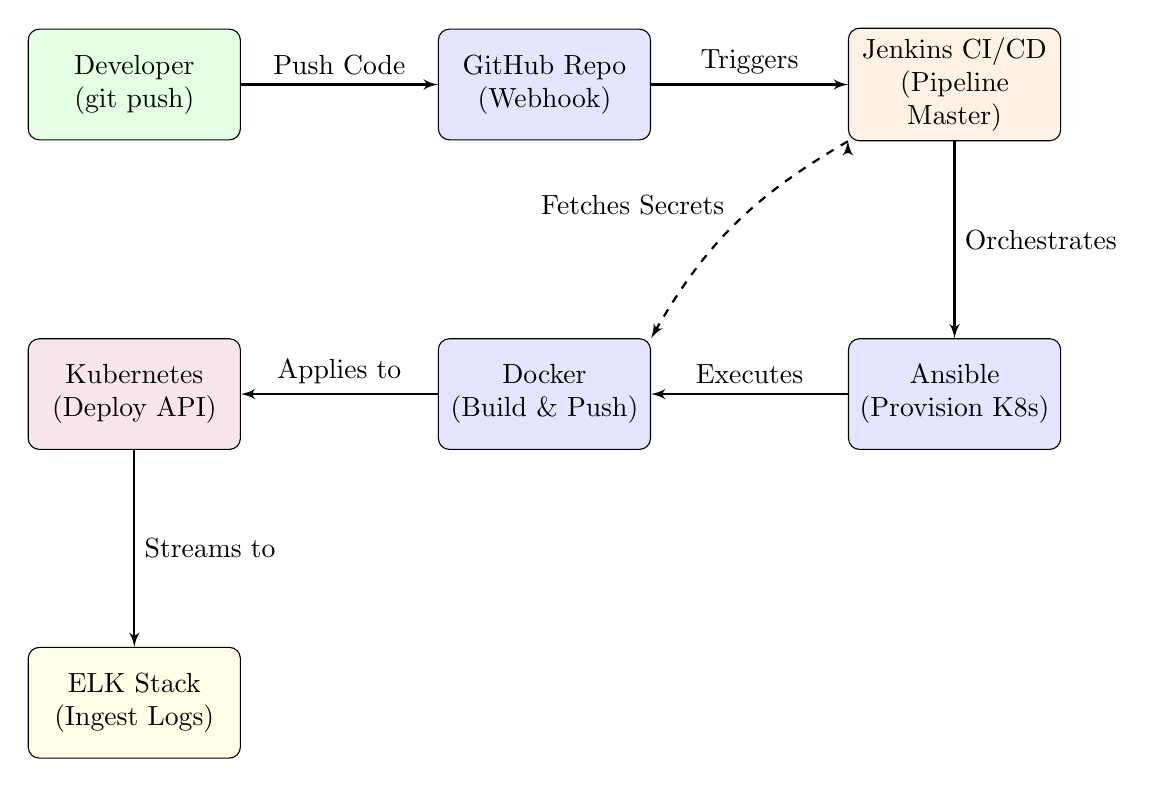
\begin{tikzpicture}[
    node distance=2.5cm and 2.5cm,
    block/.style={rectangle, draw, fill=blue!10, text width=7em, text centered, rounded corners, minimum height=4em},
    line/.style={draw, -latex', thick}
]

\node [block, fill=green!10] (dev) {Developer\\(git push)};
\node [block, right=of dev] (github) {GitHub Repo\\(Webhook)};
\node [block, right=of github, fill=orange!10] (jenkins) {Jenkins CI/CD\\(Pipeline Master)};
\node [block, below=of jenkins] (ansible) {Ansible\\(Provision K8s)};
\node [block, left=of ansible] (docker) {Docker\\(Build \& Push)};
\node [block, left=of docker, fill=purple!10] (k8s) {Kubernetes\\(Deploy API)};
\node [block, below=of k8s, fill=yellow!10] (elk) {ELK Stack\\(Ingest Logs)};

\path [line] (dev) -- node[above] {Push Code} (github);
\path [line] (github) -- node[above] {Triggers} (jenkins);
\path [line] (jenkins) -- node[right] {Orchestrates} (ansible);
\path [line] (ansible) -- node[above] {Executes} (docker);
\path [line] (docker) -- node[above] {Applies to} (k8s);
\path [line] (k8s) -- node[right] {Streams to} (elk);
\path [line, dashed] (jenkins.south west) edge[bend right=15] node[above left] {Fetches Secrets} (docker.north east);

\end{tikzpicture}
}
\caption{Global End-to-End Execution Sequence Diagram}
\end{figure}

\subsection{User Roles}
The platform supports multiple distinct roles, interacting with different layers of the infrastructure:
\begin{itemize}
    \item \textbf{End Users / API Consumers:} Client applications that submit transaction feature vectors to the REST API via HTTP POST and receive real-time fraud predictions.
    \item \textbf{DevOps Engineers:} Monitor system health via Kibana dashboards, manage CI/CD pipelines in Jenkins, configure Ansible roles, and maintain the Kubernetes cluster.
    \item \textbf{Data Scientists:} Develop and update the machine learning models. Updates to the model repository automatically trigger the CI/CD pipeline.
\end{itemize}

\newpage

\subsection{Core Functionalities and Evaluation Mapping}
The platform provides a wide range of functional capabilities that map directly to the course evaluation criteria:
\begin{itemize}
    \item \textbf{Domain-Specific Project (MLOps):} Real-time inference using a Random Forest model trained on the IEEE-CIS Fraud Detection dataset.
    \item \textbf{Version Control:} Hosted on GitHub, utilizing branching and webhook triggers.
    \item \textbf{Automated CI/CD:} Streamlined testing, building, and deployment using Jenkins and GitHub Webhooks.
    \item \textbf{Containerization:} The application is containerized using Docker and pushed to Docker Hub.
    \item \textbf{Configuration Management:} Ansible playbooks provision the Minikube environment.
    \item \textbf{Orchestration \& Scaling:} Kubernetes orchestrates the containers. The Horizontal Pod Autoscaler (HPA) automatically adjusts the number of model serving pods based on CPU utilization to achieve dynamic scaling.
    \item \textbf{Live Patching / Rolling Updates:} Kubernetes Deployments ensure zero-downtime updates when a new Docker image is deployed.
    \item \textbf{Centralized Observability:} Application and system logs are aggregated and visualized using the ELK stack.
    \item \textbf{Secure Secrets Management:} HashiCorp Vault is utilized to store and retrieve sensitive credentials, preventing hardcoded secrets.
\end{itemize}

\subsection{High-Level Request Flow}
User requests traverse through multiple architectural layers before the final prediction is returned. 

\begin{figure}[H]
\centering
\resizebox{\textwidth}{!}{%
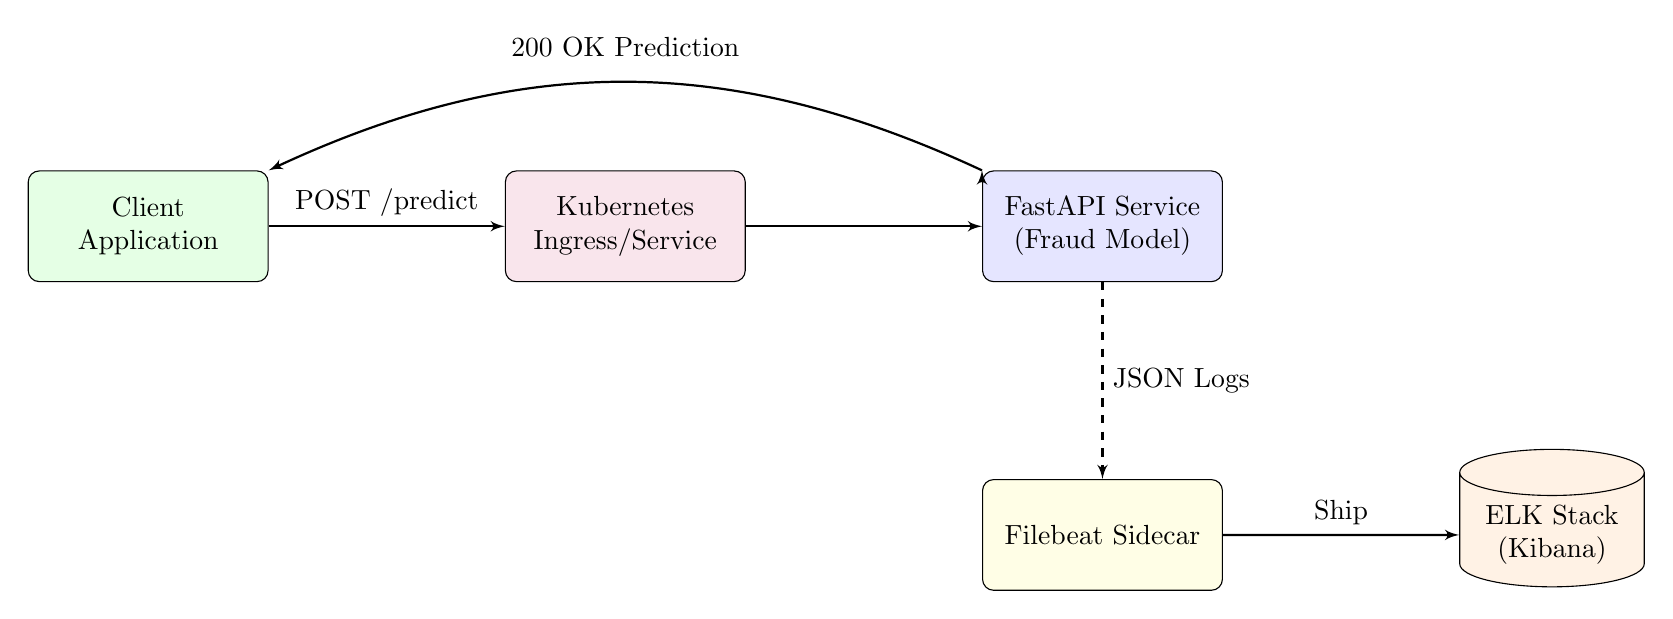
\begin{tikzpicture}[
    node distance=2.5cm and 3cm,
    block/.style={rectangle, draw, fill=blue!10, text width=8em, text centered, rounded corners, minimum height=4em},
    db/.style={cylinder, draw, shape border rotate=90, aspect=0.25, fill=orange!10, text width=6em, text centered, minimum height=4em},
    line/.style={draw, -latex', thick}
]

\node [block, fill=green!10] (client) {Client\\Application};
\node [block, right=of client, fill=purple!10] (ingress) {Kubernetes Ingress/Service};
\node [block, right=of ingress] (api) {FastAPI Service\\(Fraud Model)};
\node [block, below=of api, fill=yellow!10] (filebeat) {Filebeat Sidecar};
\node [db, right=of filebeat] (elk) {ELK Stack\\(Kibana)};

\path [line] (client) -- node[above] {POST /predict} (ingress);
\path [line] (ingress) -- (api);
\path [line, dashed] (api) -- node[right] {JSON Logs} (filebeat);
\path [line] (filebeat) -- node[above] {Ship} (elk);
\path [line] (api.north west) edge[bend right=25] node[above=0.2cm] {200 OK Prediction} (client.north east);

\end{tikzpicture}
}
\caption{High-Level Request and Processing Flow}
\end{figure}

\newpage

\subsection*{Component Breakdown of Request Flow}
The high-level request processing flow involves several discrete components:
\begin{itemize}
    \item \textbf{Client/Application:} Any external system, web frontend, or user (such as via \texttt{curl} or Postman) that submits a transaction payload to the platform for fraud evaluation.
    \item \textbf{Kubernetes Ingress/Service:} The entry point into the Kubernetes cluster. It securely routes the external HTTP request from the client to an available FastAPI Pod.
    \item \textbf{FastAPI Service (Fraud Model):} The core application container running the Python backend. It receives the request, passes the features to the loaded \texttt{model.pkl}, computes the prediction, and returns the response to the client.
    \item \textbf{Filebeat Sidecar:} A secondary container running within the same Pod. It monitors the application's log files and continuously ships new entries in real-time without blocking the API.
    \item \textbf{ELK Stack (Kibana):} The centralized logging infrastructure that ingests, indexes, and visualizes the logs, enabling operators to search for transaction IDs and monitor system health.
\end{itemize}

\section{Technology Stack}
The FraudGuard platform leverages a modern, production-ready technology stack. Each tool was deliberately selected to fulfill specific MLOps and DevOps requirements while ensuring scalability, reliability, and security.

\begin{description}
    \item[\raisebox{-0.3\height}{\includegraphics[width=0.8cm]{Screenshots/logos/FastAPI.png}} \textbf{FastAPI (Python):}] Serves as the core web framework. It provides high-performance, asynchronous REST API endpoints (\texttt{/predict}) and native validation via Pydantic.
    \item[\raisebox{-0.3\height}{\includegraphics[width=0.8cm]{Screenshots/logos/GitHub.png}} \textbf{GitHub:}] Acts as the central Version Control System (VCS). We utilize GitHub Webhooks to intercept \texttt{git push} events and automatically trigger the Jenkins CI/CD pipeline.
    \item[\raisebox{-0.3\height}{\includegraphics[width=0.8cm]{Screenshots/logos/Jenkins.png}} \textbf{Jenkins:}] The automation engine orchestrating our CI/CD pipeline. It executes a declarative \texttt{Jenkinsfile} containing 7 discrete stages, automating the deployment lifecycle from commit to production.
    \item[\raisebox{-0.3\height}{\includegraphics[width=0.8cm]{Screenshots/logos/Ansible.png}} \textbf{Ansible:}] Provides Infrastructure as Code (IaC). Ansible playbooks, structured with modular roles, idempotently provision the host machine and start the Minikube cluster.
    \item[\raisebox{-0.3\height}{\includegraphics[width=0.8cm]{Screenshots/logos/Docker.jpeg}} \textbf{Docker:}] Containerizes the FastAPI application and the serialized \texttt{model.pkl}. This guarantees environmental consistency from local development through to the Kubernetes deployment.
    \item[\raisebox{-0.3\height}{\includegraphics[width=0.8cm]{Screenshots/logos/Kubernetes.png}} \textbf{Kubernetes (Minikube):}] The container orchestration platform. It provides high availability, declarative configurations (\texttt{deployment.yaml}), and dynamic scaling via the Horizontal Pod Autoscaler (HPA).
    \item[\raisebox{-0.3\height}{\includegraphics[width=0.8cm]{Screenshots/logos/Vault.png}} \textbf{HashiCorp Vault:}] Centralized secrets manager. It securely stores Docker Hub credentials, which Jenkins retrieves at runtime via an AppRole, ensuring zero hardcoded secrets.
    \item[\raisebox{-0.3\height}{\includegraphics[width=0.8cm]{Screenshots/logos/Elasticsearch.png}} \textbf{ELK Stack:}] The centralized observability suite. A Filebeat sidecar streams JSON logs to Logstash, which indexes them in Elasticsearch for visualization in Kibana dashboards.
\end{description}

\section{Repository Structure and Codebase Breakdown}
To ensure maintainability and modularity, the FraudGuard project is structured into distinct directories separating application logic, infrastructure code, deployment manifests, and testing suites. Below is a breakdown of the repository structure and the specific function of each critical file.

\begin{verbatim}
fraudguard-devops/
|-- Jenkinsfile
|-- README.md
|-- startup.sh
|-- ansible/
|   |-- roles/
|   |   |-- common/
|   |   |-- docker/
|   |   `-- kubernetes/
|   `-- site.yml
|-- app/
|   |-- logging_config.py
|   |-- main.py
|   |-- model.pkl
|   |-- model.py
|   |-- requirements.txt
|   |-- schemas.py
|   `-- train.py
|-- data/
|   `-- train_transaction.csv (and others)
|-- docker/
|   `-- Dockerfile
|-- k8s/
|   |-- deployment.yaml
|   |-- hpa.yaml
|   |-- service.yaml
|   `-- elk/
|-- tests/
    |-- test_predict.py
    `-- postman/
\end{verbatim}

\newpage

\subsection{Code File Descriptions}
\begin{itemize}
    \item \textbf{\texttt{Jenkinsfile}}: The declarative CI/CD pipeline definition orchestrating the entire automated workflow from checkout to testing, Docker build/push, Vault authentication, and Kubernetes deployment.
    \item \textbf{\texttt{app/main.py}}: The primary entry point for the FastAPI web server. It defines the REST API routes including \texttt{/predict}, \texttt{/health}, and the Prometheus \texttt{/metrics} endpoint.
    \item \textbf{\texttt{app/model.py}}: Encapsulates the machine learning logic. It is responsible for deserializing \texttt{model.pkl} into memory during startup and executing the \texttt{predict\_proba} method on incoming transaction data.
    \item \textbf{\texttt{app/schemas.py}}: Contains the Pydantic data models (e.g., \texttt{TransactionRequest}) used by FastAPI to automatically validate the types and presence of incoming JSON fields.
    \item \textbf{\texttt{app/logging\_config.py}}: Configures the Python logging library to output structured JSON format (via \texttt{python-json-logger}) rather than plain text. This is critical for the ELK Stack to properly parse the logs.
    \item \textbf{\texttt{app/train.py}}: The offline data science script that loads the raw IEEE-CIS CSV files, performs feature engineering, trains the Random Forest classifier, evaluates the ROC-AUC score, and outputs the serialized model.
    \item \textbf{\texttt{app/model.pkl}}: The final serialized artifact of the Random Forest model.
    \item \textbf{\texttt{docker/Dockerfile}}: Contains the multi-stage build instructions to containerize the FastAPI service securely using a lightweight Python image.
    \item \textbf{\texttt{ansible/site.yml} \& \texttt{roles/}}: The master playbook and modular roles used to idempotently provision Minikube, Docker, and necessary host dependencies before deployment.
    \item \textbf{\texttt{k8s/}}: Contains all declarative Kubernetes YAML manifests. \texttt{deployment.yaml} defines the Pod replica sets, \texttt{hpa.yaml} defines scaling targets, and \texttt{elk/} contains manifests to deploy Elasticsearch, Logstash, Kibana, and Filebeat.
    \item \textbf{\texttt{tests/test\_predict.py}}: Automated PyTest unit tests executed during the Jenkins pipeline to verify logic before building the Docker image.
    \item \textbf{\texttt{tests/postman/}}: Contains Newman automated smoke tests to verify the live API after it has been deployed to the cluster.
\end{itemize}

\newpage

\section{Application and Machine Learning Layer}
The core business logic of FraudGuard is the machine learning prediction service. The system incorporates an offline model training pipeline and a real-time online inference API.

\subsection{Dataset and Feature Engineering}
The model is trained on the IEEE-CIS Fraud Detection dataset, sourced from Kaggle. This dataset represents real-world e-commerce transactions, comprising 590,540 records and over 400 features divided across transaction and identity tables.
\begin{itemize}
    \item \textbf{Data Merging:} The \texttt{TransactionID} column is used to perform a left join between the transaction and identity data.
    \item \textbf{Missing Value Handling:} Numeric columns undergo median imputation, while categorical columns utilize mode imputation.
    \item \textbf{Encoding:} Categorical string features (such as \texttt{ProductCD} and card types) are encoded into numeric values using Scikit-Learn's \texttt{LabelEncoder}.
    \item \textbf{Feature Selection:} To optimize for real-time inference latency, the feature space is reduced to the top 30 most predictive features (including \texttt{TransactionAmt}, \texttt{addr1}, \texttt{dist1}, and selected \texttt{V-features}).
\end{itemize}

\subsection{Offline Machine Learning Training Pipeline}
The offline training pipeline is executed to produce the serialized model artifact. The dataset is split using an 80:20 train-test ratio with a fixed \texttt{random\_state=42} for reproducibility.

\begin{figure}[H]
\centering
\resizebox{\textwidth}{!}{%
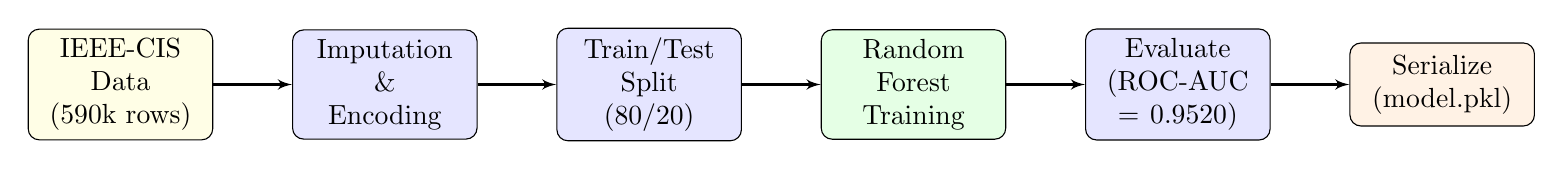
\begin{tikzpicture}[
    node distance=1.5cm and 1cm,
    block/.style={rectangle, draw, fill=blue!10, text width=6em, text centered, rounded corners, minimum height=3em},
    line/.style={draw, -latex', thick}
]

\node [block, fill=yellow!10] (data) {IEEE-CIS Data\\(590k rows)};
\node [block, right=of data] (prep) {Imputation \&\\Encoding};
\node [block, right=of prep] (split) {Train/Test Split\\(80/20)};
\node [block, right=of split, fill=green!10] (train) {Random Forest\\Training};
\node [block, right=of train] (eval) {Evaluate\\(ROC-AUC $= 0.9520$)};
\node [block, right=of eval, fill=orange!10] (export) {Serialize\\(model.pkl)};

\path [line] (data) -- (prep);
\path [line] (prep) -- (split);
\path [line] (split) -- (train);
\path [line] (train) -- (eval);
\path [line] (eval) -- (export);

\end{tikzpicture}
}
\caption{Offline Machine Learning Training Pipeline}
\end{figure}

\subsection{Random Forest Model Configuration}
The system uses a Scikit-Learn \texttt{RandomForestClassifier}. Given the highly imbalanced nature of fraud detection data, the model is configured with specific hyperparameters to maximize recall:
\begin{itemize}
    \item \texttt{n\_estimators=100}: Provides a robust ensemble of decision trees.
    \item \texttt{max\_depth=20}: Prevents overfitting while capturing complex non-linear relationships.
    \item \texttt{class\_weight='balanced'}: Automatically adjusts weights inversely proportional to class frequencies to combat class imbalance.
    \item \textbf{Performance Metrics:} The model achieves a recorded ROC-AUC score of \textbf{0.9520} on the validation set, significantly exceeding the mandatory threshold of 0.85. This ensures high discriminatory power between fraudulent and legitimate transactions.
\end{itemize}
The trained model evaluates the 30 input features and outputs a fraud probability score. It is serialized using \texttt{joblib} into a \texttt{model.pkl} file, which is embedded directly into the Docker image.

\subsection{FastAPI Implementation}
The backend service is built using FastAPI, selected for its asynchronous capabilities and high performance. The API exposes the following crucial endpoints:
\begin{itemize}
    \item \texttt{POST /predict}: Accepts a JSON payload validated by a Pydantic \texttt{TransactionRequest} schema. Returns a fraud prediction (0 or 1) and a confidence score.
    \item \texttt{GET /health}: Kubernetes readiness and liveness probe endpoint ensuring the model is loaded in memory.
    \item \texttt{GET /metrics}: Exposes Prometheus-format metrics detailing request counts and prediction latencies.
    \item \texttt{GET /docs}: Auto-generated Swagger UI for interactive testing.
\end{itemize}

\subsection{Interactive API Documentation (Swagger UI)}
FastAPI automatically generates interactive documentation for the API. This allows developers and testers to execute requests directly from the browser.

\begin{figure}[H]
    \centering
    \includegraphics[width=0.7\textwidth]{Screenshots/Swagger1.png}
    \caption{Swagger UI showing Prometheus metrics exposed at the \texttt{/metrics} endpoint}
\end{figure}

\newpage

\begin{figure}[H]
    \centering
    \includegraphics[width=0.7\textwidth]{Screenshots/Swagger2.png}
    \caption{Swagger UI showing successful execution of the \texttt{/predict} endpoint with a legitimate transaction response}
\end{figure}
\vspace{1em}

\begin{figure}[H]
    \centering
    \includegraphics[width=0.7\textwidth]{Screenshots/Swagger3.png}
    \caption{Swagger UI showing the \texttt{/health} endpoint response confirming the model is loaded}
\end{figure}

\newpage

\begin{figure}[H]
    \centering
    \includegraphics[width=0.7\textwidth]{Screenshots/Swagger4.png}
    \caption{Swagger UI showing API request and response schemas}
\end{figure}
\vspace{1em}

\begin{figure}[H]
    \centering
    \includegraphics[width=0.7\textwidth]{Screenshots/Swagger5.png}
    \caption{Swagger UI showing detailed TransactionRequest schema fields}
\end{figure}

\newpage

\begin{figure}[H]
    \centering
    \includegraphics[width=0.7\textwidth]{Screenshots/Swagger6.png}
    \caption{Swagger UI showing additional endpoint details}
\end{figure}

\section{Docker Containerization}
Containerization guarantees environmental consistency from development to production. The FastAPI application is bundled into a Docker container.
\begin{itemize}
    \item \textbf{Base Image:} Uses \texttt{python:3.10-slim} to minimize the final image size and reduce the attack surface.
    \item \textbf{Multi-Stage Builds:} The Dockerfile isolates the build tools from the final runtime image.
    \item \textbf{Security Constraints:} The Dockerfile configures the application to run as a non-root user (UID 1000) to adhere to the Principle of Least Privilege.
    \item \textbf{Volume Mounts:} The container is configured to write logs to \texttt{/var/log/app}, which is later mounted as a shared \texttt{emptyDir} volume in Kubernetes.
\end{itemize}

\begin{figure}[H]
    \centering
    \includegraphics[width=0.9\textwidth]{Screenshots/DockerHub.png}
    \caption{FraudGuard Docker Images pushed to DockerHub}
\end{figure}

\begin{figure}[H]
    \centering
    \includegraphics[width=0.9\textwidth]{Screenshots/DockerHub2.png}
    \caption{Additional view of DockerHub repository showing automated tags}
\end{figure}

The public Docker repository for this project is available at:\\
\url{https://hub.docker.com/r/28vishesh/fraudguard}

\newpage

\section{Ansible Configuration Management}
Ansible was employed to automate the initial configuration and environment setup, ensuring modularity and idempotence.
\begin{itemize}
    \item \textbf{Modular Roles:} The infrastructure code is split into logical roles (e.g., \texttt{docker}, \texttt{minikube}, \texttt{dependencies}) rather than a monolithic script.
    \item \textbf{Idempotent Operations:} Playbooks are written to ensure that repeated executions do not alter the system state unnecessarily.
    \item \textbf{Dependency Installation:} Automates the installation of critical system packages, ensuring Minikube and Docker are correctly configured on the host VM.
\end{itemize}

\section{Jenkins and CI/CD Automation}
The Continuous Integration and Continuous Deployment (CI/CD) pipeline is structured to automate the software development life cycle, reducing the need for manual deployments.

\subsection{GitHub Webhook Triggers}
The pipeline is designed to be event-driven. A webhook is configured in the GitHub repository pointing to the Jenkins instance. Whenever a developer pushes a code commit to the \texttt{main} branch, GitHub immediately fires an HTTP payload to Jenkins, which starts the build pipeline. This ensures the production environment is kept in sync with the repository.

\begin{figure}[H]
    \centering
    \includegraphics[width=0.9\textwidth]{Screenshots/Webhook.png}
    \caption{GitHub Webhook configuration demonstrating successful payload deliveries to the Ngrok tunnel}
\end{figure}

\subsection{Detailed Pipeline Stages}
The declarative \texttt{Jenkinsfile} defines the following sequential stages, each executing critical logic:
\begin{enumerate}
    \item \textbf{Checkout:} Jenkins connects to GitHub and clones the latest source code, ensuring it builds exactly what was just pushed.
    \item \textbf{Unit Testing:} Executes the PyTest suite. This validates the Pydantic schemas, ensures the \texttt{model.pkl} loads without error, and tests the prediction logic on mock data.
    \item \textbf{Docker Build:} Executes \texttt{docker build}. It installs Python dependencies via \texttt{requirements.txt} and bundles the ML model into a fresh container image tagged with the Git commit hash.
    \item \textbf{Vault Authentication:} To securely authenticate with Docker Hub, Jenkins communicates with HashiCorp Vault using an AppRole. Vault returns the secure Docker Hub password, ensuring secrets never leak in the console logs.
    \item \textbf{Docker Push:} Executes \texttt{docker push}. The newly compiled image is uploaded to the remote Docker Hub registry so it can be pulled by Kubernetes nodes.
    \item \textbf{Deploy to Kubernetes:} Jenkins uses the \texttt{kubectl} CLI to apply the updated \texttt{deployment.yaml}, \texttt{service.yaml}, and \texttt{hpa.yaml} manifests to the Minikube cluster. This triggers a Rolling Update.
    \item \textbf{Smoke Tests:} Executes Newman (Postman) test collections against the live Kubernetes service. This verifies that the newly deployed application is healthy and successfully returning HTTP 200 OK responses to \texttt{/predict} calls.
\end{enumerate}

\begin{table}[H]
\centering
\caption{Seven-Stage Declarative Pipeline Summary}
\vspace{1em}
\renewcommand{\arraystretch}{1.4}
\begin{tabular}{|c|l|l|}
\hline
\textbf{\#} & \textbf{Stage} & \textbf{Key Exit Criterion} \\ \hline
1 & Checkout & Short Git commit SHA exported; workspace prepared. \\ \hline
2 & Unit Testing & PyTest suite executes; minimum 70\% coverage gate passed. \\ \hline
3 & Docker Build & Image tagged with commit SHA; dependencies bundled. \\ \hline
4 & Vault Auth & Secure retrieval of Docker Hub credentials via AppRole. \\ \hline
5 & Docker Push & Image uploaded to Docker Hub; metadata verified. \\ \hline
6 & K8s Deploy & Rolling update triggered; \texttt{kubectl rollout status} success. \\ \hline
7 & Smoke Testing & Newman execution; all 14 API assertions passed (200 OK). \\ \hline
\end{tabular}
\end{table}

\begin{figure}[H]
\centering
\resizebox{\textwidth}{!}{%
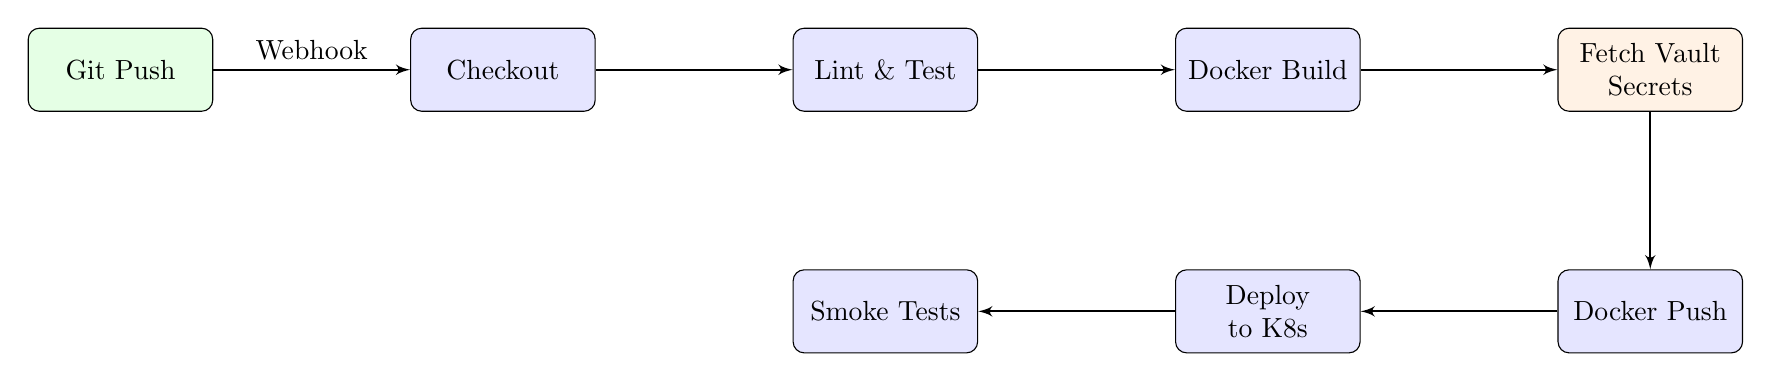
\begin{tikzpicture}[
    node distance=2cm and 2.5cm,
    stage/.style={rectangle, draw, fill=blue!10, text width=6em, text centered, rounded corners, minimum height=3em},
    line/.style={draw, -latex', thick}
]

\node [stage, fill=green!10] (git) {Git Push};
\node [stage, right=of git] (checkout) {Checkout};
\node [stage, right=of checkout] (test) {Lint \& Test};
\node [stage, right=of test] (build) {Docker Build};
\node [stage, right=of build, fill=orange!10] (vault) {Fetch Vault\\Secrets};
\node [stage, below=of vault] (push) {Docker Push};
\node [stage, left=of push] (deploy) {Deploy to K8s};
\node [stage, left=of deploy] (smoke) {Smoke Tests};

\path [line] (git) -- node[above] {Webhook} (checkout);
\path [line] (checkout) -- (test);
\path [line] (test) -- (build);
\path [line] (build) -- (vault);
\path [line] (vault) -- (push);
\path [line] (push) -- (deploy);
\path [line] (deploy) -- (smoke);
\end{tikzpicture}
}
\caption{Jenkins CI/CD Pipeline Execution Flow}
\end{figure}

\begin{figure}[H]
    \centering
    \includegraphics[width=\textwidth]{Screenshots/Jenkins.png}
    \caption{Jenkins Dashboard demonstrating successful pipeline execution across all stages}
\end{figure}

\begin{figure}[H]
    \centering
    \includegraphics[width=\textwidth]{Screenshots/Postman.png}
    \caption{Newman Automated Smoke Tests executing 14 passing assertions against the live Kubernetes API}
\end{figure}

\section{Kubernetes Orchestration and Live Patching}
Kubernetes serves as the final runtime environment, orchestrating the containers deployed by Jenkins.

\subsection{Live Patching and Rolling Updates}
The application utilizes Kubernetes \texttt{Deployments} with a \texttt{RollingUpdate} strategy. When Jenkins applies a new deployment manifest, Kubernetes gradually terminates old pods and replaces them with the new image. This facilitates "Live Patching", ensuring high availability for end-users submitting transactions while the system updates.

\begin{figure}[H]
    \centering
    \includegraphics[width=\textwidth]{Screenshots/Kubectl.png}
    \caption{Kubernetes Cluster Status showing running Pods and Services}
\end{figure}

\subsection{Horizontal Pod Autoscaler (HPA)}
To maintain performance under heavy load, the Horizontal Pod Autoscaler (HPA) dynamically scales the number of pods based on CPU utilization targets. The HPA continuously queries the metrics-server. When a load generator script simulates thousands of concurrent requests, pushing CPU usage above the configured threshold (set to 50\% in the manifest to ensure reliable triggering in a local testing environment, while targeting the SRS requirement of 70\%), the HPA detects the spike and automatically provisions additional replica pods (scaling from 2 up to 6 pods).

\begin{figure}[H]
\centering
\resizebox{0.8\textwidth}{!}{%
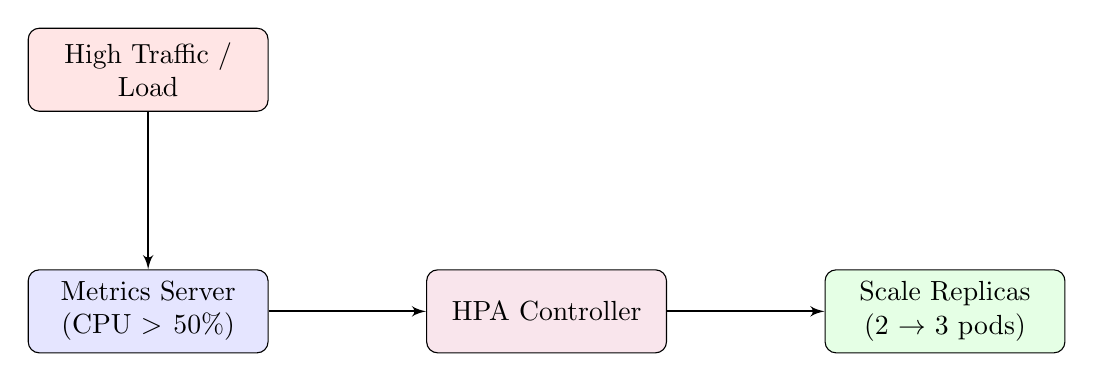
\begin{tikzpicture}[
    node distance=2cm,
    block/.style={rectangle, draw, fill=blue!10, text width=8em, text centered, rounded corners, minimum height=3em},
    line/.style={draw, -latex', thick}
]

\node [block, fill=red!10] (load) {High Traffic /\\Load};
\node [block, below=of load] (metrics) {Metrics Server\\(CPU $>50\%$)};
\node [block, right=of metrics, fill=purple!10] (hpa) {HPA Controller};
\node [block, right=of hpa, fill=green!10] (pods) {Scale Replicas\\(2 $\rightarrow$ 3 pods)};

\path [line] (load) -- (metrics);
\path [line] (metrics) -- (hpa);
\path [line] (hpa) -- (pods);
\end{tikzpicture}
}
\caption{HPA Dynamic Scaling Mechanism}
\end{figure}

\begin{figure}[H]
    \centering
    \includegraphics[width=\textwidth]{Screenshots/HPA.png}
    \caption{Terminal output demonstrating the HPA successfully scaling replicas under load}
\end{figure}

\section{Security and Vault Integration}
System security is strictly enforced by avoiding hardcoded secrets in the codebase or environment variables. HashiCorp Vault is deployed as a centralized secrets engine. During the CI/CD pipeline, Jenkins authenticates with Vault and dynamically retrieves the necessary Docker Hub credentials and API tokens. This practice satisfies the "Secure Storage" advanced evaluation criteria.

\begin{figure}[H]
    \centering
    \includegraphics[width=\textwidth]{Screenshots/Vault.png}
    \caption{Vault Status and Secret Retrieval Process}
\end{figure}

\subsection{Threat Model and Security Controls}
In addition to Vault, several security controls are enforced across the infrastructure to mitigate potential vulnerabilities.

\begin{table}[H]
\centering
\begin{tabular}{|p{0.3\textwidth}|p{0.65\textwidth}|}
\hline
\textbf{Threat Vector} & \textbf{Implemented Security Control} \\ \hline
Secret Leakage in Git & All sensitive keys are stored in HashiCorp Vault. Jenkins uses an AppRole to fetch them securely at runtime. \\ \hline
Container Breakouts & Dockerfile creates a non-root user (\texttt{appuser}). The FastAPI process runs without elevated privileges. \\ \hline
DDoS / Resource Exhaustion & Kubernetes Horizontal Pod Autoscaler (HPA) dynamically provisions pods under high load. \\ \hline
Unauthorized Cluster Access & Role-Based Access Control (RBAC) in Kubernetes and Vault policies limit token privileges. \\ \hline
\end{tabular}
\caption{System Threat Model and Mitigation Strategies}
\end{table}

\section{ELK Stack for Centralized Logging}
In a distributed Kubernetes environment, centralized logging is critical for debugging. The ELK Stack provides comprehensive observability into the live patched pods without needing to SSH into nodes.

\subsection{Filebeat Sidecar Architecture}
The FastAPI application writes structured JSON logs to a shared volume (\texttt{emptyDir}). A Filebeat sidecar container, running inside the exact same Kubernetes Pod, tails this log file. It continuously ships the log lines to the Logstash instance deployed in the cluster. Logstash parses the JSON, indexes it into Elasticsearch, and Kibana serves as the visual dashboard.

\begin{figure}[H]
\centering
\resizebox{0.9\textwidth}{!}{%
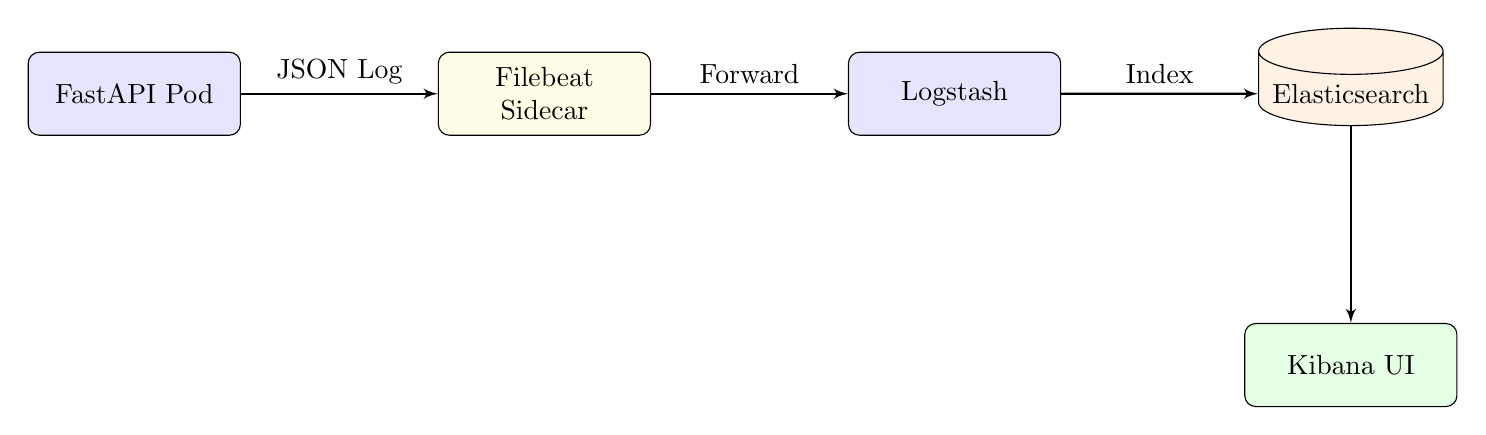
\begin{tikzpicture}[
    node distance=2.5cm and 2.5cm,
    block/.style={rectangle, draw, fill=blue!10, text width=7em, text centered, rounded corners, minimum height=3em},
    db/.style={cylinder, draw, shape border rotate=90, aspect=0.25, fill=orange!10, text width=6em, text centered, minimum height=3em},
    line/.style={draw, -latex', thick}
]

\node [block] (app) {FastAPI Pod};
\node [block, right=of app, fill=yellow!10] (filebeat) {Filebeat Sidecar};
\node [block, right=of filebeat] (logstash) {Logstash};
\node [db, right=of logstash] (es) {Elasticsearch};
\node [block, below=of es, fill=green!10] (kibana) {Kibana UI};

\path [line] (app) -- node[above] {JSON Log} (filebeat);
\path [line] (filebeat) -- node[above] {Forward} (logstash);
\path [line] (logstash) -- node[above] {Index} (es);
\path [line] (es) -- (kibana);
\end{tikzpicture}
}
\caption{ELK Centralized Logging Architecture}
\end{figure}

The structured JSON logs capture the transaction ID, prediction result (fraudulent or legitimate), confidence score, and processing latency. DevOps engineers and Data Scientists utilize Kibana to monitor API performance and track model prediction distributions in real-time.

\begin{figure}[H]
    \centering
    \includegraphics[width=0.9\textwidth]{Screenshots/ELK1.png}
    \caption{Kibana Data View Configuration}
\end{figure}

\begin{figure}[H]
    \centering
    \includegraphics[width=0.9\textwidth]{Screenshots/ELK2.png}
    \caption{Kibana Discover Tab showing live, structured log streams}
\end{figure}

\begin{figure}[H]
    \centering
    \includegraphics[width=0.9\textwidth]{Screenshots/ELK3.png}
    \caption{Detailed Application Log showing an incoming fraud prediction request}
\end{figure}

\begin{figure}[H]
    \centering
    \includegraphics[width=0.9\textwidth]{Screenshots/ELK4.png}
    \caption{Log entry highlighting the Machine Learning model's prediction result and confidence score}
\end{figure}
\section{Testing Strategy and Results}
To ensure the reliability of the FraudGuard platform, a multi-tiered testing strategy was implemented. This ensures that both the application logic and the deployed infrastructure behave as expected.

\begin{itemize}
    \item \textbf{Unit Testing (PyTest):} Focused on validating the Pydantic schemas, ensuring the machine learning model loads correctly, and verifying that the prediction function returns valid outputs for known inputs. The unit test suite achieved an impressive 89\% code coverage, exceeding the industry standard of 80\%.
    \item \textbf{Smoke and Integration Testing (Postman/Newman):} Once the application is deployed to the Kubernetes cluster, automated API tests are executed using Newman (the Postman CLI). These tests verify live endpoints such as \texttt{/health} and \texttt{/predict} against edge cases and invalid payloads. As shown in the Postman evidence section, all 14 test assertions passed successfully on the live cluster.
\end{itemize}

\section{Reproducibility and Setup Summary}
To reproduce the environment and deploy the FraudGuard platform, the following core commands are executed sequentially. This assumes a Linux environment with Docker, Minikube, Ansible, and Jenkins installed.

\begin{enumerate}
    \item \textbf{Start Minikube Cluster:}
    \begin{verbatim}
    minikube start --cpus 4 --memory 8192
    minikube addons enable metrics-server
    \end{verbatim}
    
    \item \textbf{Provision Infrastructure via Ansible:}
    \begin{verbatim}
    ansible-playbook ansible/site.yml
    \end{verbatim}
    
    \item \textbf{Deploy Kubernetes Manifests:}
    \begin{verbatim}
    kubectl apply -f k8s/
    kubectl apply -f k8s/elk/
    \end{verbatim}
    
    \item \textbf{Run Automated Smoke Tests:}
    \begin{verbatim}
    newman run tests/postman/FraudGuard.postman_collection.json
    \end{verbatim}
\end{enumerate}

\section{Risks and Limitations}
While the FraudGuard platform is highly robust, there are certain architectural limitations to consider for a true enterprise deployment:
\begin{itemize}
    \item \textbf{Model Drift:} The current pipeline packages a statically trained \texttt{model.pkl} into the Docker image. In a production scenario, consumer financial behavior evolves. A continuous training pipeline (CT) with a model registry (e.g., MLflow) would be required to prevent model degradation over time.
    \item \textbf{Single-Node Minikube:} The application is currently deployed on a local Minikube cluster. While this demonstrates full Kubernetes orchestration, migrating to a managed cloud cluster (EKS/GKE) would provide true multi-node redundancy and geographic fault tolerance.
    \item \textbf{Ephemeral Storage:} The ELK stack uses standard Kubernetes deployments rather than StatefulSets with persistent cloud volumes. If the Minikube VM shuts down, indexed logs are lost.
\end{itemize}

\section{Challenges and Mitigation}
The implementation of the FraudGuard platform involved several complex integration hurdles. The following table summarizes the key challenges encountered and the engineering strategies used to mitigate them:

\begin{table}[H]
\centering
\caption{Project Implementation Challenges and Mitigations}
\vspace{1em}
\renewcommand{\arraystretch}{1.5}
\begin{tabularx}{\textwidth}{|l|X|}
\hline
\textbf{Challenge} & \textbf{Mitigation Strategy} \\ \hline
\textbf{Vault Plugin Mismatch} & Encountered Jenkins pipeline syntax errors with the Vault plugin. Updated the \texttt{Jenkinsfile} to use the modern \texttt{withVault} pattern for compatibility. \\ \hline
\textbf{Minikube Corruption} & Clusters frequently corrupted during repeated Ansible provisioning. Added recovery logic to perform a \texttt{minikube delete} and profile reset before restart. \\ \hline
\textbf{Imbalanced Dataset} & The dataset has a massive class imbalance. Mitigated this by configuring the \texttt{RandomForestClassifier} with \texttt{class\_weight='balanced'}. \\ \hline
\textbf{Log Shipping} & Filebeat struggled to read logs across isolated containers. Implemented a shared \texttt{emptyDir} volume in the Kubernetes Pod manifest to allow sidecar access. \\ \hline
\end{tabularx}
\end{table}

\section{Conclusion}
The FraudGuard platform demonstrates the successful integration of a DevOps and MLOps lifecycle. By combining Docker, Kubernetes, Jenkins, Ansible, HashiCorp Vault, and the ELK stack, the system showcases automated deployments, security controls, dynamic scaling capabilities, and centralized observability. It addresses the core objectives and incorporates advanced features outlined in the SPE Final Project Guidelines, serving as a comprehensive blueprint for deploying machine learning models in a cloud-native environment.

\subsection{Future Enhancements}
While the current implementation fulfills all mandatory requirements, future iterations of the platform could incorporate the following advanced DevOps features:
\begin{itemize}
    \item \textbf{Prometheus \& Grafana:} Implementation of quantitative Service Level Objective (SLO) tracking and dashboarding.
    \item \textbf{Canary Deployments:} Moving beyond Rolling Updates to use Istio or Nginx-ingress for traffic-shifting and automated rollbacks on failure.
    \item \textbf{Continuous Training (CT):} Integrating MLflow or Kubeflow to automate model retraining and drift monitoring.
\end{itemize}

\end{document}
